
\section{Influence of hyperparameters}\label{params}

In order to investigate how the network's learning behavior depends on the size of the training set and other hyperparameters, such as the learning rate, batch size and number of neurons in the hidden layer, we used the \textit{costOverEpochs()} function and the script \textit{costDiffParams()}.
The \textit{costOverEpochs()} function is very similar to the \textit{trainNetwork()} function. It trains a neural network with one hidden layer and a given set of network parameters for
a fixed number of epochs. Thereafter it evaluates the cost function after each epoch on the test dataset and returns the epoch-evolution of the cost function. The script \textit{costDiffParams} is then used to generate cost vs. epoch curves for different parameter bundles. In the course of this, only one network parameter is changed at a time while the others (variables with the suffix 'Usual' in the script) are kept constant.

Figure \ref{fig:costTestset_sizeTrain} shows the cost curves for different numbers of training inputs (details in the plot). One recognizes that for a larger training set the cost decreases more faster and saturates at a lower absolute cost value, which meets our expectations.

Figure \ref{fig:costTestset_eta} shows the cost curves for different learning rates, whereby the whole training set was used to train the network. For a small learning rate of 0.6 the cost decreases more slowly compared to larger learning rates and is comparably smooth, but also saturates at a higher absolute cost value. Whereas the curve remains smooth for a learning rate of 1.0, it gets bumpy for larger learning rates which is likely due to overshooting (the learning rate is so high, that it overshoots the optimal point).

Figure \ref{fig:costTestset_batchSize} depicts the cost curves for different batch sizes. For a very small batch size of just 2 training inputs, the cost rapidly decreased after the first epoch but exhibits the most bumpy behaviour. This is probably due to individual training inputs being too much weighted during the adjustment of the network parameters, which results in the temporary optimization of the weights and biases just on these inputs. For a (comparably large) batch size of 250 training inputs, the cost decreases more slowly than with smaller batches. It also doesn't seem to be saturated after 20 epochs. The degregation of gradient descent based feedforward neural networks trained with a large batch size is a common issue and the reason is still investigated\footnote{N. S. Keskar, \textit{et al.}, \textit{On Large-Batch Training for Deep Learning: Generalization Gap and Sharp Minima}, ICLR (\textbf{2017})}.

Figure \ref{fig:costTestset_numNeurons} shows the cost curves for a varying number of neurons in the hidden layer. NEW PLOT

\newpage
\begin{figure}[h!]
\centering
    \centering
    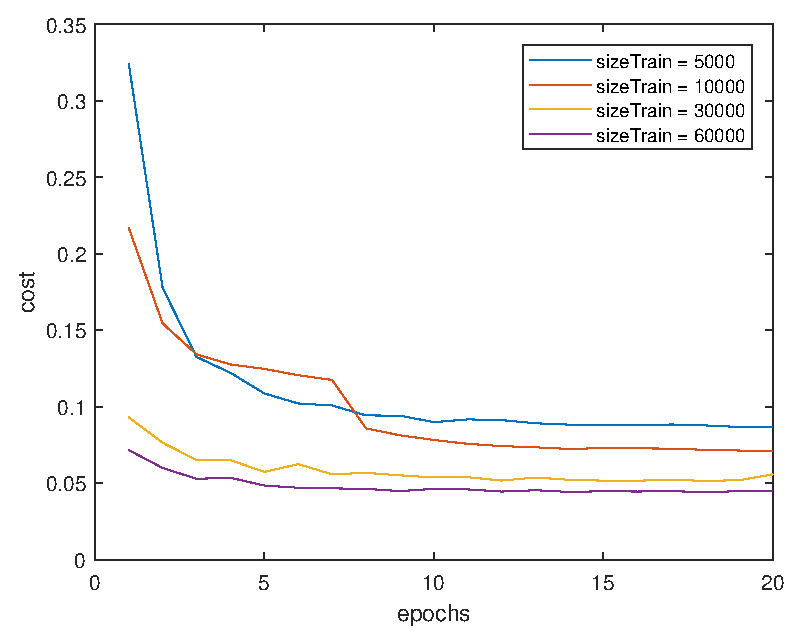
\includegraphics[width=0.92\textwidth]{test_src/img/20epochs/costOverEpochs_sizeTrain}
    \caption{Cost over 20 epochs for different sizes of the training set, a learning rate of 3, a batch size of 10 and 30 neurons in the hidden layer}
    \label{fig:costTestset_sizeTrain}
\end{figure}
\begin{figure}[h!]
\centering
    \centering
    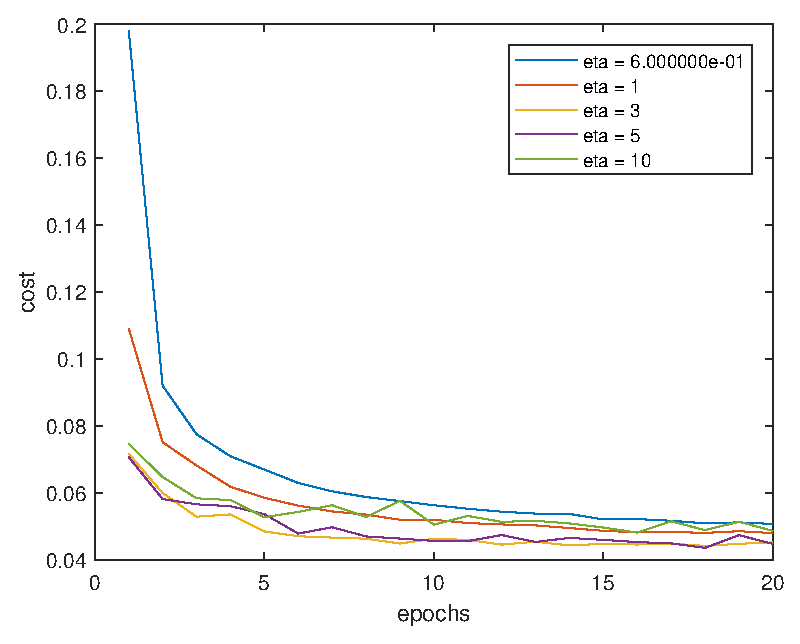
\includegraphics[width=0.92\textwidth]{test_src/img/20epochs/costOverEpochs_eta}
    \caption{Cost over 20 epochs for different learning rates, the whole training set (60000 inputs), a batch size of 10 and 30 neurons in the hidden layer}
    \label{fig:costTestset_eta}
\end{figure}

\newpage
\begin{figure}[h!]
\centering
    \centering
    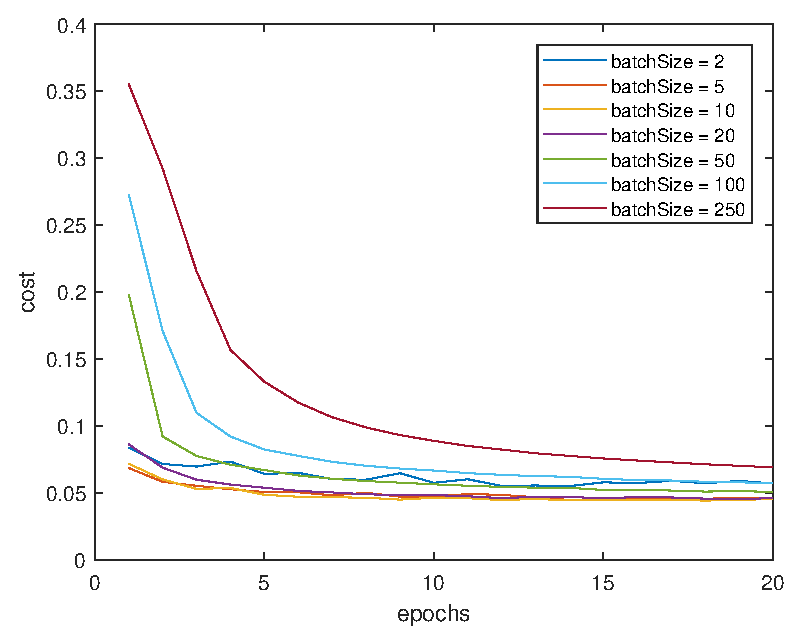
\includegraphics[width=0.91\textwidth]{test_src/img/20epochs/costOverEpochs_batchSize}
    \caption{Cost over 20 epochs for different batch sizes, the whole training set (60000 inputs), a learning rate of 3 and 30 neurons in the hidden layer}
    \label{fig:costTestset_batchSize}
\end{figure}
\begin{figure}[h!]
\centering
    \centering
    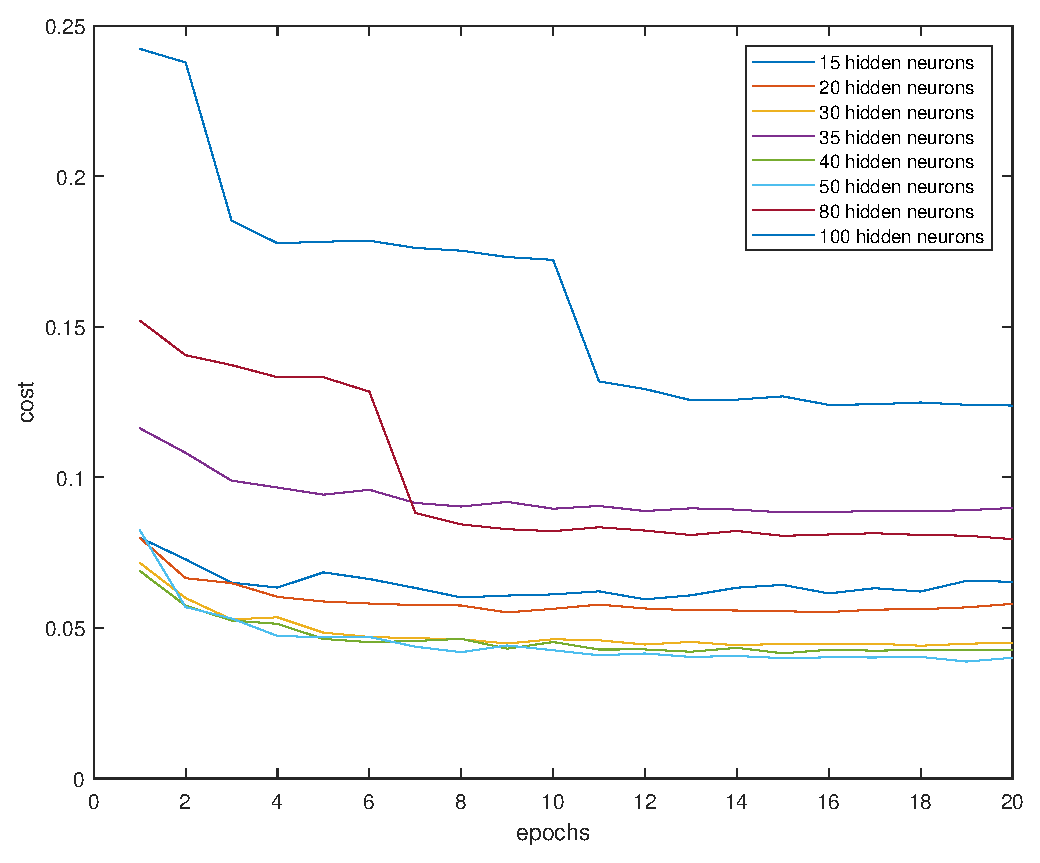
\includegraphics[width=0.91\textwidth]{test_src/img/20epochs/costOverEpochs_numNeurons}
    \caption{Cost over 20 epochs for numbers of neurons in the hidden layer, the whole training set (60000 inputs) and a batch size of 10}
    \label{fig:costTestset_numNeurons}
\end{figure}

%In addition for the number of neurons, the computation time needed to train the network and evaluate the cost function is plotted.

\section{Performance on MNIST Database}\label{detRate}
